\documentclass[11pt]{article}
%\usepackage{isolatin1}
%\usepackage{adjustbox}
\usepackage{epsfig}
\usepackage{setspace}
\usepackage[english]{babel}
%\usepackage[latin1]{inputenc}
\usepackage[usenames,dvipsnames]{xcolor}
\usepackage{setspace}
\usepackage{float}
\usepackage{amssymb}
\usepackage{epsfig}
\usepackage{cite}
\usepackage{graphicx}
\usepackage{tabularx} % in the preamble
\usepackage{caption}
%\usepackage{enumitem}
\usepackage{url}
\usepackage{listings}


\usepackage[latin1]{inputenc} % 
\bibliographystyle{plain}

\oddsidemargin 0pt  % was 38
\evensidemargin 0pt % was 38
\marginparwidth 0pt % was 68
% 
\topmargin 50pt   % was 27
\headheight 0pt  % was 12
\headsep 0pt     % was 25
%\footheight 0pt  % was 12
\footskip 30pt   % was 30
 
\textwidth 470pt      % was 390pt
\textheight 600.5pt  % was 536.5

\floatstyle{ruled}
\newfloat{algoritmo}{thp}{loa}
\floatname{algoritmo}{Algoritmo}
 
% Colors on or off: Pick ONE
\newcommand{\ifColorText}[2]{\textcolor{#1}{#2}}  % Colors ON
%\renewcommand{\ifColorText}[2]{{#2}}                   % Colors OFF

% To turn comments OFF simply comment out  the \Commentstrue line
\newif\ifComments
%\Commentstrue

\ifComments
\newcommand{\chek}[1]{\noindent\textcolor{red}{Check: {#1}}}
\newcommand{\marcio}[1]{\noindent\textcolor{ForestGreen}{Marcio: {#1}}}
\newcommand{\guido}[1]{\noindent\textcolor{magenta}{Guido: {#1}}}
\newcommand{\rem}[1]{\noindent\textcolor{red}{Removed: {#1}}}
\newcommand{\new}[1]{\noindent\textcolor{blue}{ {#1}}}
\newcommand{\ed}[1]{\noindent\textcolor{red}{ {#1}}}
\newcommand{\short}[1]{\noindent\textcolor{blue}{ {#1}}}
\else
\newcommand{\chek}[1]{}
\newcommand{\marcio}[1]{}
\newcommand{\guido}[1]{}
\newcommand{\rem}[1]{}
\newcommand{\new}[1]{#1}
\newcommand{\ed}[1]{}
\newcommand{\short}[1]{}
\fi

\input{abaco.tex}

\begin{document}

\thispagestyle{empty}

\begin{minipage}[tl]{31mm}
  \ABACO{1}{9}{6}{9}{1}
\end{minipage}
\hspace*{3mm}
\begin{minipage}[tl]{12cm}
  \begin{center} 
    {
      {\Large Computer Systems Laboratory \\
        Department of Computer Systems \\ } 
      {\large Institute of Computing \\
        University of Campinas}
    }
  \end{center}
\end{minipage}

\vfill
{\LARGE
  \begin{center}
      \textbf{Support for Parallel Scan in OpenMP}

  \end{center}
}
\vfill
{\large

\hspace{4cm}
\begin{tabular}{|rl|}

    \hline 
%        Processo: & {\bf 99/09462-8} \\ \hline \hline 
           Student: & Eder Maicol Gomez Zegarra \\
                  & \emph{egomezz@students.ic.unicamp.br} \\  \hline \hline
          
      Advisor: & Prof. Dr. Guido Costa Souza de Ara�jo \\
                  & \emph{guido@ic.unicamp.br} \\ \hline \hline
      Co-Advisor: & Prof. Dr. Marcio Machado Pereira \\
                        & \emph{mpereira@ic.unicamp.br} \\ \hline \hline
        Content: &    Abstract \\
                 & 1. Introduction \\
                 & \,\,\,\,\,\,\,\,1.1. Parallel Computation\\
                 & \,\,\,\,\,\,\,\,1.2. Prefix Sums Problem\\
                 & 2. Related Works \\
                 & 3. Work Proposal\\
                 & \,\,\,\,\,\,\,\,3.1. Design Scan clause in OpenMP\\
                 & \,\,\,\,\,\,\,\,3.2. Scan Implementation in OpenCL\\
                 & \,\,\,\,\,\,\,\,3.3. Implementation Algorithm\\
                 & \,\,\,\,\,\,\,\,3.4. Operator Generalization\\
                 & 4. Preliminary Experimental Results\\
                 & 5. Work Plan\\
                 & References\\ \hline 
\end{tabular}
\newpage

\begin{spacing}{1.5}


%============================================
%----------RESUMO---------------------------------------
%============================================

\begin{center}
{\LARGE Abstract}
\end{center}

Prefix Sum or also called Prefix  Scan problem aims to compute all the
partial sums  of a vector  of values resulting  in a vector,  the same
size as  the original  vector, where  each element is  the sum  of the
preceding  elements in  the original  vector up  to the  corresponding
position.  There  are  two  versions of  Prefix  Scan:  inclusive  and
exclusive.  For an  inclusive  scan,  the result  is  the  sum of  all
preceding  values as  well as  the value  of the  element itself.  The
exclusive  version   does  not  include   the  value  of   the  vector
element. \new{In  this proposal we}\rem{The future work} will take
into account both versions.

\rem{\\Besides Prefix  Scan  is  used  in  different  algorithms  as
Quicksort, Lexical  Analysis, String  Comparation, etc.  Therefore the
creation of a parallel Scan as  a clause in OpenMP could help to
improve  the performance  of these  algorithms and  other applications
than may arise.   In this context, the propose for  the master project
is implement a  clause scan for OpenMP with  parallel algorithms using
Cuda C and OpenCL.}

\new{Prefix  Scan is  used  in different  algorithms as  Quicksort,
  Lexical Analysis, String Comparation, etc. This research propose the
  creation of a parallel version  of Prefix Scan, therefore referenced
  by Parallel Scan,  as a clause in OpenMP to  improve the performance
  of these algorithms and another algorithms that may appear.  In the context of the
  master project  research, we  will design  and implement  the OpenMP
  scan clause in the {\it gpuclang project}, a framework developed at
  Unicamp based  on Clang/LLVM compiler targeting GPU-based
  heterogeneous systems with support of OpenCL.}



\clearpage

\section{Introduction}
\label{section:intro}

\subsection{Parallel Computation}

The invention  of the microprocessor has  changed radically scientific
development, the computational ability of the microprocessors has made
that problems that were unsolvable or unrealistic in the past, now can
be solved easier.

For more than half century, the development of the microprocessors has
followed the Moore's law, which mentions that the number of transistor
could increase exponentially (doubling  approximately) every two years
\cite{moorelaw}. The current microprocessors can reach a peak speed as
high  as several  Giga-FLOPS (floating  point operations  per second),
compared to 5000  simple additions and subtractions per  second of the
first computed invented in 1946 \cite{eniac}.

The computers are faster over time. Consequently the users want to
resolve more complex problems that require compute more
information. No  only the  scientist require better  performance in
computation of information in their problems (e.g.,  weather, physics,
and biological processes), also  the commercial applications that need
 fast information processing  for some solutions (e.g., video
conferencing, computer-aided medical diagnosis, and virtual
reality). At  same time  the speed of  a uni-processor  computer is
limited by  its physics dimensions  and the number of  the transistors
\cite{processorlimitations}. For these reasons, multi-processor 
computers were  designed.

However, nowadays the most existing algorithms designed are to work in
serial form  (uni-processor). Whereby these algorithms  do not exploit
the resources  of the others  processors.  The basic idea  of parallel
computing is to carry out  multiple tasks simultaneously for which the
algorithms should be designed so that they can use all the processors.
However, we  must considerer  than in the  foreseeable future  we will
probably work with hundreds of cores. This  is an  issue 
because  if silicon vendors and  application developers cannot give  
better performance to users with new  hardware, the whole hardware and
software market will go from selling  new products, to simply 
maintaining existing product
lines~\cite{state}.  Algorithms  such  as  finite-state machines  and
other   intrinsically  serial   algorithms  are   most  suitable   for
single-core CPUs running at  high frequencies. Embarrassingly parallel
algorithms such as Monte Carlo simulations, on the other hand, benefit
greatly from many accelerator cores running at a lower frequency. Most
applications consist of  a mixture of such serial  and parallel tasks,
and will  ultimately perform best on  heterogeneous architectures. The
optimal type  and composition of  processors, however, will  vary from
one  application  to  another.   With the  recent  emphasis  on  green
computing, it becomes essential to use all possible resources at every
clock  cycle. Both  academia and industry realize  that serial performance
has  reached  its  zenith,  leading  to  an  increased  focus  on  new
algorithms   that  can   benefit  from   parallel  and   heterogeneous
architectures. Further insight into these different architectures, and
their implications on algorithm performance, is essential in algorithm
design and for  application developers to bridge the  gap between peak
performance and  experienced performance.  The field  of heterogeneous
computing  covers a  large  variety of  architectures and  application
areas,  and there  is  currently  no unified  theory  to encompass  it
all. Fair comparisons of the architectures are therefore difficult.

For a better understanding,  Heterogeneous computing \cite{hc} refers to systems that use more than one kind of processor. These are multi-core systems that  gain  performance  not  just   by  adding  cores,  but  also  by incorporating specialized processing capabilities to handle particular
tasks.  Heterogeneous   System  Architecture  (HSA)   systems  utilize
multiple processor  types (typically  CPUs and  GPUs), usually  on the
same silicon die, to give you the best of both worlds: GPU processing,
apart from its well-known 3D graphics rendering capabilities, can also
perform mathematically intensive computations on very large data sets,
while CPUs can run the operating system and perform traditional serial
tasks.

\marcio{Maicol, falta a referencia hc, acima}

\rem{Essentially, in the  future work of master theses  will be implemented
the algorithm of Prefix Scan in  parallel version such that it is used
as OpenMP clause.}

\subsection{Prefix Sums Problem}

In computer science, the prefix sum, cumulative sum, inclusive scan,
or simply scan is defined by (see~\cite{ScanAsPrimitive}):

\new{
\begin{description}
\item[\ ]{Given a  binary associative operator}\ $\oplus$
\item[\ ]{and an ordered set of  n elements}\ $[a_{0}, a_{1}, ... ,a_{n-1}]$
\item[\ ]{return  the ordered set}\ 
 $[ a_{0}, a_{0} \oplus a_{1}, ... ,a_{0} \oplus  a_{1} \oplus ... \oplus  a_{n-1}]$
\end{description}}

Here, more details if the binary operator was the addition:\\
Define  a sequence  of number  $x[0], x[1],  ..., x[n]$  and a  second
sequence of  numbers $y[0],  y[1], ..., y[n]$  the operator  scan will
calculate the second sequence as follows:

\begin{eqnarray}
    y[0] = x[0]\nonumber\\
    y[1] = x[0] + x[1]\nonumber\\
    y[2] = x[0] + x[1]+ x[2]\nonumber\\
    ...\nonumber
\end{eqnarray}

Which can be simplified to:

\begin{equation}
    y[i] = \sum_{j=0}^{i} x[j] 
\end{equation}

Prefix  sums   are  trivial  to   compute  in  sequential   models  of
computation, by  using the formula $y[i]  = y[i-1] + x[i]$  to compute
each  output   value  in   sequence  order.   This  is   calculate  in
$\mathcal{O}(n)$ time complexity.

However, despite their  ease of computation, prefix sums  are a useful
primitive  in  Sorting  Algorithms (Radix  Sort,  Quick-sort,  Counting
Sort),  Lexical Analysis,  String  Comparison, Polynomial  Evaluation,
Stream  Compaction  and  Building   Histograms  and  Data  Structures.
Abstractly, a prefix  sum requires only a  binary associative operator
$\oplus$,  making it  useful  for many  applications from  calculating
well-separated pair decompositions of points to string processing.

In the next example, we will present how can we use scan operator to 
parallelize quick-sort algorithm, as we remember quick-sort has three 
main parts, the first one is to pick a pivot, the second one is sort 
the elements lower equals than the pivot to the left and the greater to
the right of the pivot. The last part is sort the left and right part 
recursively using the steps one and two, see the Figure \ref{quicksort}.

To parallelize quick-sort we have to use array filter technique, this 
is one interesting application so that all elements satisfying a 
particular property.
One example where we want to do this is during the pivot step of Quicksort: After selecting a pivot element, we want to move all elements that are less than this selected pivot to the beginning of the array (and all elements greater than the pivot to the end ? but that is basically the same problem).
To accomplish our filtering, we first create another array where each entry is 1 if the element satisfies the condition says to keep the corresponding element of the original array and 0 otherwise. Then we compute all prefix sums of this array. For each element that satisfies the condition says to keep, the corresponding prefix sum indicates where it should be placed into the new array; so finally we can just place each kept number into the indicated index.

\begin{figure}[H]
	\centering
	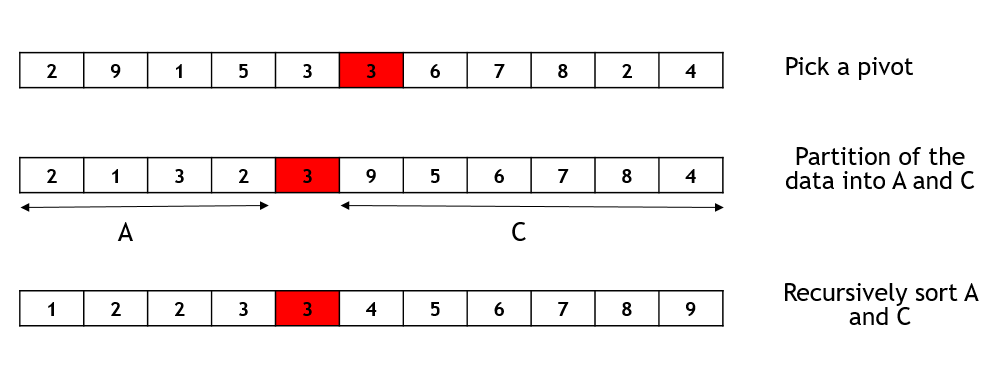
\includegraphics[width=0.8\textwidth]{quicksort.png}
	\captionsetup{justification=centering}
	\caption{Example of the three main steps of quicksort Algorithm}
	\label{quicksort}
\end{figure}

To illustrated array filter technique we can show the next example:
Suppose that we have a vector $A$ and condition, our condition refers to get
all the elements greater than 10.\\
$A \: = \: <17, 4, 6, 8, 11, 5, 13, 19, 0, 24>$ and we desire  $<17, 11, 13, 19, 24>$\\
As we mentioned before, as first step, we perform a vector of bits where
the $i$ element is 1 if satisfy the condition 0 otherwise, in our case.\\
$input \:\: <17, 4, 6, 8, 11, 5, 13, 19, 0, 24>$\\
$bits \:\: <1, 0, 0, 0, 1, 0, 1, 1, 0, 1>$\\
Then perform a vector bitsum with the operator scan.\\
$bitsum \:\: <1, 1, 1, 1, 2, 2, 3, 4, 4, 5> $\\
As last step, to every with value of 1 in the vector $bits$ we saved the value
from the vector input and we placed in the position that we have in the
vector $bitsum$, finally we get the desire vector.\\
$output \:\: <17, 11, 13, 19, 24>$\\

Prefix Scan  will work with  any associative combining  operation. The
most common  is addition  (and we'll  use this  on examples),  but the
operations of multiplication, maximum, minimum, and logical operations
(such  as AND,  OR,  and  Exclusive OR)  are  all  possible, too.  The
combining operation  used does not  need to be commutative  because of
the  fixed order  that is  used  to combine  elements.  Consider,  for
instance, this  simple C code,  which evaluate  the Sums in  the input
array:

\vspace{0.5cm}

\begin{lstlisting}
void prefix_sum_array (float* input, float* output, int length) {
    output[0] = input[0];
    for (int i = 1; i < length; i++) 
        output[i] = output[i-1] + input[i];
}
\end{lstlisting}


\section{Related Works}
\label{sec:TrabalhosRelacionados}

W.  Daniels and  Guy L.  Steele Jr.  \cite{dataparallel} developed  an
approach  to  parallelize many  serial  algorithms  of size  $N$  whit
complexity  $O(N)$,  these  algorithms  were resolved  in  $O(log  N)$
time. Many of  these algorithms seemed to have only  a serial solution
however with  the machine developed  by W. Daniels  $The$ $Connection$
$Machine$ \cite{themachine} was possible to improve these algorithms.

The Connection Machine systems  \cite{themachine} had either 16,364 or
65,536 processors, each with 4,096 bits  of memory. The system had two
parts: a  front-end computer of  the usual  von Neumann style,  and an
array of  Connection Machine processors.  Each processor in  the array
had a small  amount of local memory, and the  front end, the processor
array looks like a memory.

One  of the  algorithms  that was  solved  in \cite{dataparallel}  was
$Sum \: of \: an  \: array \: of \: N \: numbers$.   It was one of the
first solutions  designed to  be executed in  parallel. To  solve this
problem   the   array   was   organized   as   binary   tree.   Figure
\ref{Sumof8Elemtns} illustrates the  method on an array  of 8 elements
named $x_{0}$ through $x_{7}$.
\begin{figure}[h]
   \centering
   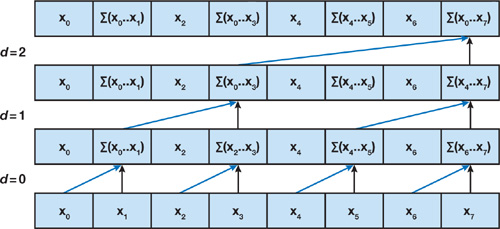
\includegraphics[width=0.8\textwidth]{sumOfArray8.jpg}
   \caption{Computing the Sum of an Array of 8 Elements}
   \label{Sumof8Elemtns}
\end{figure}

In this algorithm, for purposes  of simplicity, the number of elements
to be summed is  assumed to be an integral power of  two. There are as
many processors  as elements, and  the statement \textbf{for all  k in
  parallel  do  s  od}  causes  all processors  to  execute  the  same
statement s in synchrony, but the variable k has a different value for
each processor, namely, the index of that processor within the array.

\begin{lstlisting}
int Computing_Sum_of_Array(int *x, int n){
    for(int j = 1 ; j <= log(n) ; j++)
        for(int k = 0 ; k < n ; k++)
	    if( (k+1) % (2 ^ j) == 0 )
	        x[k] = x[k - 2 ^ (j-1)] + x[k];
				
    return x[n-1];
}
\end{lstlisting}

At the end of the process, $x_{n-1}$ contains the sum of the n elements.\\
One second algorithm  was \textbf{All Partial Sums of  an Array} where
we already know this problem as Prefix Sum or Scan. Looking the simple
summation             algorithm            mentioned             above
$Sum \: of \: an \: array \: of \: N \: numbers$.  We see that most of
the processors  are idle most  of the  time: During iteration  j, only
n/21 processors  are active, and,  indeed, half of the  processors are
never used.  However, by putting  the idle  processors to good  use by
allowing  more  processors to  operate,  the  summation algorithm  can
compute all partial  sums of the array  in the same amount  of time it
took to  compute the  single sum. In  defining $\sum_{j}^{k}$  to mean
$\sum_{i=j}^{k}x_{i}$, note  that $\sum_{j}^{k}$ +  $\sum_{k+1}^{m}$ =
$\sum_{j}^{m}$. The  partial-sums algorithms replaces each  $x_{k}$ by
$\sum_{0}^{k}$:  that  is,  the  sum of  all  elements  preceding  and
including $x_{k}$. In Figure \ref{PartialSums}, this process is illustrated for an
array of 8 elements.


\begin{figure}[h]
   \centering
   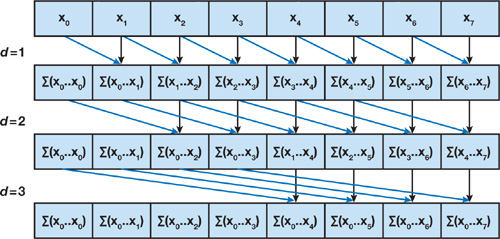
\includegraphics[width=0.8\textwidth]{PartialSumsOfArray.jpg}
   \caption{Computing Partial Sums of an Array of 8 Elements}
   \label{PartialSums}
\end{figure}

\begin{lstlisting}
void Computing_Partial_Sums_of_Array(int *x, int n){
    for(int j = 1 ; j <= log(n) ; j++)
	for(int k = 0 ; k < n ; k++)
	    if( k >= 2 ^ j )
	        x[k] = x[k - 2 ^ (j-1)] + x[k];
}
\end{lstlisting}

The only difference between this algorithm and the first one is the
test in the if statement in this algorithm, that determines whether a
processor will perform the assignment. This algorithm keeps more
processors active: During step $j$, $n$ $-$ $2^{j-1}$ processors are
in use; after step $j$, element number $k$ has become $\sum_{a}^{k}$
where $a$ $=$ $max(0, k - 2^{j} + 1)$.

As we were defined before the operation Scan and therefore this
technique can be generalized from summation to any associative binary
operator. Some obvious choices are product, maximum, minimum, and
logical AND, OR, and EXCLUSIVE OR.

Guy E. Blelloch in his work \cite{ScanAsPrimitive} outlined a study of
the effect  of including certain  scan operations as such  "unit time"
primitives in the  PRAM (Parallel Random Access  Machine) models. This
operator  was  used in  five  algorithms  and  that used  improve  the
asymptotic running time of these  algorithms by $O(log N)$ factor over
EREC (Exclusive Read Exclusive Write) model  and some by an $O(log N)$
factor over  the CRCW (Concurrent  Read Concurrent Write)  model.  The
algorithms  improved  with  the  used of  the  scan  were  radix-sort,
Quicksort,  Minimum-spanning-tree, line-drawing  and  merging. We  can
appreciate in this work than the operation \textbf{Scan} could help us
to  improve a  variety  of algorithms  where is  possible  to use  the
operator.

Daniel Horn in his work on  the book $GPU$ $Gems$ $2$ \cite{GPUGems2},
present a  scan operator using GPU  device based in Hillis  and Steele
work \cite{dataparallel} to  solve the next problem: Assume  we have a
data set  with arbitrary values and  we wish to extract  all positives
values. The use of scan operator  allowed to obtain a running count of
the number  of null records, and  then a search and  gather to compact
them, for a final running time of $O(N log N)$.\\
To solve the problem,
for each value of  the input vector was modified, if  the value of the
vector was  positive then this value  was maker as zero  otherwise was
marked as  one. In the  next figure \ref{scangpu1} we  illustrated how
the algorithm works to get the number of null  records and the vector
of partial sums than be used  to compact the positive numbers, we just
concentrate in the first part of the algorithm (Scan Operator).

\begin{figure}[H]
   \centering
   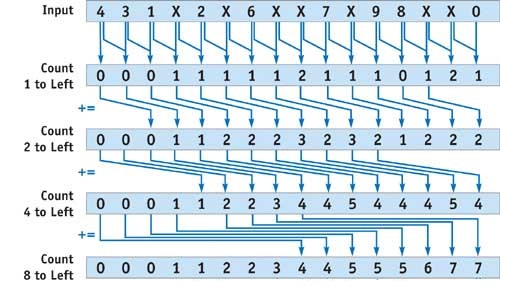
\includegraphics[width=0.8\textwidth]{ScanGPU1.jpg}
   \caption{Computing the number of null records}
   \label{scangpu1}
\end{figure}

As we can see in the Figures \ref{scangpu1} and \ref{PartialSums}, the
algorithms are the same, except  that in the Figure \ref{scangpu1} the
algorithm is  used to  particular problem.  This work  was one  of the
first implementations for the operator Scan in GPU.

Three years  later in the  the book $GPU$  $Gems$ $3$, Mark  Harris et
al. \cite{GPUGems3}  design a better  algorithm to Scan  operator than
was  presented  by   Horn  \cite{GPUGems2}  than  was   based  in  the
implementation by Hillis and  Steele \cite{dataparallel}, he mentioned
than the implementation  of the algorithm was not  the optimal because
the number of operations is $O(log N)$ meanwhile in the serial version
the number of  operation was $O(N)$ hence designed  an algorithm based
on the one  presented by Blelloch \cite{ScanAsPrimitive}.  The goal of
this  work  was  to avoid  the  extra  factor  $log  N$ in  number  of
operations by the algorithm mentioned above. To solve this problem was
used an algorithm pattern often used $balanced trees$.
The idea is to build a balanced binary tree on the input data and
sweep it to and from the root to compute the prefix sum. A binary tree
with $n$ leaves has $d$ $=$ $log n$ levels, and each level $d$ has
$2^{d}$ nodes. If we perform one add per node, then we will perform
$O(n)$ adds on a single traversal of the tree.

The tree we  build is not an  actual data structure, but  a concept we
use  to  determine  what  each  thread   does  at  each  step  of  the
traversal. The algorithm consists of  two phases: the reduce phase and
the down-sweep phase.  In the reduce phase, we traverse  the tree from
leaves to root  computing partial sums at internal nodes  of the tree,
as shown in Figure \ref{scanreduce}. This  is also known as a parallel
reduction, because after  this phase, the root node (the  last node in
the array) holds the sum of all nodes in the array.

\begin{figure}[H]
   \centering
   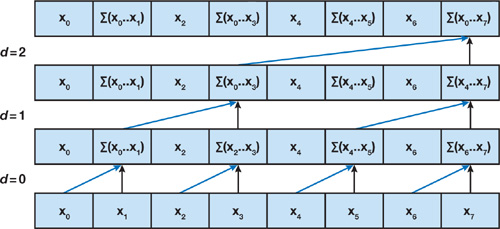
\includegraphics[width=0.8\textwidth]{ScanReduce.jpg}
   \captionsetup{justification=centering}
   \caption{An Illustration  of the  Up-Sweep, or  Reduce, Phase  of a
     Work-Efficient Sum Scan Algorithm}
   \label{scanreduce}
\end{figure}

In the down-sweep phase, we traverse back down the tree from the root,
using the  partial sums  from the  reduce phase to  build the  scan in
place on  the array.  We start by  inserting zero at  the root  of the
tree, and on each step, each node  at the current level passes its own
value to its left child, and the sum of its value and the former value
of  its left  child to  its right  child. The  down-sweep is  shown in
Figure \ref{scandown}.

\begin{figure}[H]
   \centering
   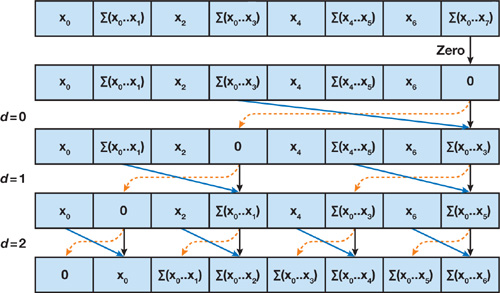
\includegraphics[width=0.7\textwidth]{ScanDown.jpg}
   \captionsetup{justification=centering}
   \caption{An   Illustration  of   the   Down-Sweep   Phase  of   the
     Work-Efficient Parallel Sum Scan Algorithm}
   \label{scandown}
\end{figure}

The total of  number of operation are $O(n)$ (it  performs $2 * (n-1)$
adds and $n - 1$ swaps); therefore it is work-efficient and, for large
arrays,  should perform  much better  than the  previous presented  in
\cite{GPUGems2}.   The work  concluded than  the scan  operation is  a
simple  and  powerful  parallel  primitive   with  a  broad  range  of
applications. This work explained  an efficient implementation
of scan using CUDA, which achieves a significant speedup compared to a
sequential implementation on a fast CPU. Also in the present work, the
algorithm was tested in  many problems (Stream Compaction, Summed-Area
Tables, Radix Sort, Merge Sorted Chunks) getting good results compared
to other implementations.

Thijs Wiefferink in  2015 published his work  \cite{ScanOpenCL}, where he
implemented  a version  mentioned in  above \cite{GPUGems3}  in OpenCL
where it is  more complicated. He improved the  algorithm about Branch
divergence,  which occurs  when threads  that execute  the kernel  are
forced  to   execute  different  instructions,  disturbing   the  SIMT
$(Single-Instruction, Multiple-Thread)$.\\As it is to be expected this
implementation works in Nvidia and  AMD GPU platforms, unlike previous
versions   than    just   work    in   Nvidia    GPU   \cite{GPUGems2}
\cite{GPUGems3}.\\But it  is not the  only version in  OpenCL, Shengen
Yan et.  al. \cite{ScanOpenCL2},  implemented Scan Operator  in OpenCL
too,  He  improved the  Scan  algorithm  about  the number  of  memory
accesses $(3N$ $to$ $2N)$ and how synchronization.


\section{Work Proposal}

\rem{For all the  above, we can assure than the  implementation of one
  optimized parallel scan  operator is not easy,  whereby the proposal
  of this research  is to implemented a clause in  OpenMP than perform
  the Scan  operator.  We have chosen  OpenMP because is a  high level
  language  and  to   the  programmer,  the  whole   process  will  be
  transparent.}

\new{For      all       that      has      been       shown      in
  section~\ref{sec:TrabalhosRelacionados},  we  can assure  that  the
implementation of parallel scan algorithms is not an easy task for the
programmers.  Thereby, the  aim  of  this research  is  to design  and
implement an OpenMP clause to perform the scan operation transparently
to the programmer.}

\subsection{Design Scan clause in OpenMP}

\rem{As we mentioned before, the  proposal is implemnted a clause Scan
  in  OpenMP which  leads to  time savings  for the  programmer.  This
  clause  will be  implemented in  OpenCL, where  it will  be work  in
  accordance a different parameters $(Size$ $of$ $data,$ $device$ $to$
  $use,$ $etc)$.  Below, a proposal for the clause Scan:}

\new{As  we mentioned  before, the  proposal  is to  design a  scan
  clause in  OpenMP which  leads to time  savings for  the programmer.
  The algorithms that  support this new clause will  be implemented in
  OpenCL in  accordance to the  user parameters (e.g., size  of data).
  Below, an example of the use of scan clause:}

\begin{lstlisting}
void prefix_sum (float* input, float* output, int size){
    output[0] = 0;
    #pragma omp parallel for scan(+: output)
    for (int i = 1; i < size; i++) 
	output[i] = output[i-1] + input[i-1];
}
\end{lstlisting}

In this example we show the Scan  clause and its parameters. As we can
see, the  first parameter  is the operator;  in general  this operator
could be any associative operator. The  second one is the array output
where are stored  the partial sums. \new{Note that  the first value
  of the output array must be initialized outside the loop.} \rem{also
  as we  can see the  first sentence we  have to initialize  the first
  value of the output array.}

\subsection{Scan Operator Implementation in OpenCL}

In this section we  \new{will briefly describe} \rem{mentioned} the
algorithm  to perform  the operator  Scan in  OpenCL. As  we mentioned
before, the programmer  doesn't have to worry about  this part because
for him it will be transparent.  In this \new{first} version of the
algorithm don't considered particular aspects as the size  of the
data or  the device  to use  (if the  programmer has  GPUs).  \rem{we}
\new{We will  fisrt implement}\rem{ed} a \rem{first}  version of the
  algorithm to  solve the  problem with the  limitation of  size. This
  version just work  in a block of  threads, so the size  of the input
  cant be very big. However, we  are already start designing a version
  for an  arbitrary size.  The current  algorithm was  based \rem{than
    was}   \new{in  the   algorithm}  mentioned   in  the   section
  \ref{sec:TrabalhosRelacionados}   \rem{on}   \new{and   in}   the
  work~\cite{GPUGems3}.  For  this version,  the algorithm  was tested
  up to  size  of  4092  \new{integer  elements}  getting  the
  corrects answers.

\subsection{Implementation Algorithm}
\label{implementation}
The   algorithm  to   perform  the   operator  Scan   \rem{will  have}
\new{has} the following steps:

\begin{enumerate}
	\item Identify the parameters of the clause.
	\item If the parameters are valid continue; if not, ignore the
          clause Scan and do nothing.
	\item \new{In accordance of the  parameters, choose an algorithm to
          solve. For example, if the size  of the data is greater than
          a determined  value, solve  with one  type of  algorithm; if
          not, solve with  another one. A similar case  can be applied
          for  the  last  parameter,  depending of  the  need  of  the
          programmer (exclusive or inclusive version).}
	\item Execute the chosen algorithm in OpenCL.
	\item Return the output array with the corresponding partial sums.	
\end{enumerate}

\new{These steps  are a resume of  the total algorithm that  involving many
considerations that are  not written yet. The purpose of  this list is
to give an overview of how the algorithm will be composed.}

\subsection{Operador Generalization}
\label{Generalization}
Just as we generalized our parallel sum algorithm from , we can also generalize our parallel prefix sum algorithm to work with an arbitrary operator $\oplus$. For this to work, our $\oplus$ operator must be associative, it must also have an identity element.
In the next example we will see one application of our generalization.
For the problem of polynomial evaluation we have an array of coefficients,
a number $x$ and we want to compute the value of:\\

$a_{n-1}x^{n-1} + a_{n-2}x^{n-2} + ... + a_{1}x^{1} + a_{0}x^{0}$\\

Our trick to solve the problem is to replace each element in the array with a pair. In this case, we will change element $a_{i}$ to become the pair $(a_{i}, x)$ in our new array. We 
will perform our scan on this new array of pairs using the $\oplus$ operator defined as follows:
\\\\
$(p, y) \oplus (q, z) = (p z + q, y z)$\\

Where does this come from? It's a little difficult to understand at first, but
each such pair is meant to summarize the essential knowledge needed for a
segment of the array. This segment itself represents a polynomial. The first
number in the pair is the value of the segment's polynomial evaluated for x,
while the second is xn, where n is the length of the represented segment.

But before we imagine using our parallel scan algorithm, we need first to
confirm that the operator is indeed associative.\\\\
$((a, x) \oplus (b, y)) \oplus (c, z) = (a y + b, x y) \oplus (c, z)$\\
$((a, x) \oplus (b, y)) \oplus (c, z) = ((a y + b) z + c, x y z) = (a y z + b z + c, x y z)$\\
$(a, x) \oplus ((b, y) \oplus (c, z)) = (a, x) \oplus (b z + c, y z) = (a y z + b z + c, x y z)$\\

Both associations yield the same result, so the operator is associative. Let's
look at an example to see it at work. Suppose we want to evaluate the
polynomial $x� + x� + 1$ when $x$ is 2. In this case, the coefficients of the
polynomial can be represented using the array $<1, 1, 0, 1>$. The first step of our
algorithm is to convert this into an array of pairs.

$<$ $(1, 2), (1, 2), (0, 2), (1, 2)$ $>$\\
We can then repeatedly apply our $\oplus$ operator to arrive at our result.\\
$(1, 2)\:\oplus\:(1, 2)\:\oplus\:(0, 2)\:\oplus\:(1, 2)\:=\:(1 . 2 + 1, 2 . 2)\:\oplus\:(0, 2)\: \oplus\:(1, 2)$\\
$(1, 2)\:\oplus\:(1, 2)\:\oplus\:(0, 2)\:\oplus\:(1, 2)\:=\:(3, 4)\:\oplus\:(0, 2)\:\oplus\:(1, 2)$\\
$(1, 2)\:\oplus\:(1, 2)\:\oplus\:(0, 2)\:\oplus\:(1, 2)\:=\:(3. 2 + 0, 4 . 2)\:\oplus\:(1, 2)\:=\:(6, 8)\:\oplus\:(1, 2)$\\
$(1, 2)\:\oplus\:(1, 2)\:\oplus\:(0, 2)\:\oplus\:(1, 2)\:=\:(6 . 2 + 1, 8 . 2) \:=\:(13, 16)$\\\\
So we end up with $(13, 16)$, which has the value we wanted to compute 13
as its first element: $2� + 2� + 1 = 13$.
In our computation above, we proceeded in left-to-right order as would be
done on a single processor. In fact, though, our parallel scan algorithm would
combine the first two elements and the second two elements in parallel:\\
$(1, 2) \:\oplus\: (1, 2) \:=\: (1 . 2 + 1, 2 . 2) \:=\: (3, 4)$\\
$(0, 2) \:\oplus\: (1, 2) \:=\: (0 . 2 + 1, 2 . 2) \:=\: (1, 4)$\\\\
And then it would combine these two results to arrive at $(3 . 4 + 1, 4 . 4)$
= $(13, 16)$.

\section{Preliminary Experiments Results}

\new{In  this section  we will  show  the results  of two  different
  implementations of the Scan  operator compared to a serial version. The
  first  one  is   the  algorithm  mentioned  in~\ref{implementation}
  written to  OpenCL and  the second implementation  is a  CUDA version
  based on~\cite{GPUGems3} as the first one.  Figure~\ref{char} shows
  the preliminary results that we got with these algorithms.}

\begin{figure}[H]
   \centering
   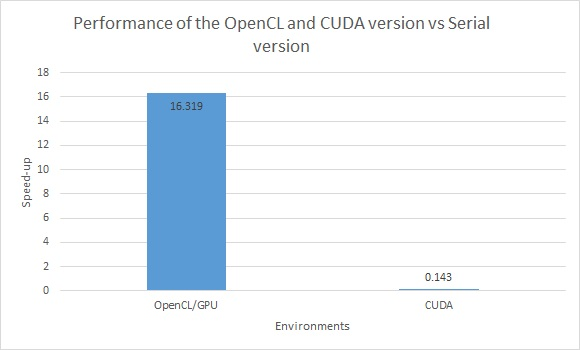
\includegraphics[width=0.8\textwidth]{Chart.jpg}
   \captionsetup{justification=centering}
   \caption{Chart of performance of Scan Operator in GCC, OpenCL and CUDA}
   \label{char}
\end{figure}

\rem{These results  are an average of  10 executions and we  can appreciate
than the  serial GCC  version is  better than  the others,  it happens
because  the size  of the  input is  small(1024) and  the cost  of the
offloading is big compare to the number of operations, to get a better
result we  have to designed an  algorithm to solve the  problem with a
bigger size of input.}

\new{These results  are an average of  10 executions and we  can appreciate
that the speedup from the OpenCL version executed in Intel GPU device
is around 16 whereby  we can ensure that the use  of the algorithm can
improve the performance of any program that uses the Scan Operator. We
need to  remember that the implementation  for now is limited  to the
size  of the  input, however  we estimate  that for  larger sizes
OpenCL version will get better speedup.}

\rem{More detailed, we can see than the worst version is in CUDA, it
happens for the reason explicated before, the cost of the offloading
to another device ($Nvidia Card$) is very expensive to the size of the
input. The cost of the OpenCL version is not so expensive because,
this version is executed on the CPU, for the future work, we will test
this version in a GPU device.}

\new{The OpenCL experiment was realized in a computer model MacBook
  with processor Intel Core i5 of 2.40 GHz, 4 cores and 4 Gb RAM. This
  computer is  equiped with a Intel  Iris GPU device with  40 parallel
  compute units  and a  maximum number of  work-items in  a work-group
  equals 512. The CUDA experiment was realized in a device GeForce GTX
  980.  For all the cases the size of the input to perform was 512. In
  the case  of CUDA version,  yet we  didn't get speedup.  However, we
  believe that happens because the size  of the input is small. We are
  designing a version  that works for an arbitrary size,  for which we
  believe we can get a better speedup.}

\section{Work Plan}

The project phases are listed below and a schedule is available in the
next section.

\begin{enumerate}
\item Study of LLVM and its IR; \label{cron:1}
\item Study Literature review; \label{cron:2}
\item Study of Scan; \label{cron:3}
\item Defense of EQM; \label{cron:4}
\item Study of OpenCL and CUDA; \label{cron:5}
\item Create a library of algorithms for use according to the parameters; \label{cron:6}
\item Implementation of Scan Clause; \label{cron:7}
\item Implementation optimizations on Scan Clause; \label{cron:8}
\item Writing an article and submitting to Congress; \label{cron:9}
\item Writing and review of dissertation; \label{cron:10}
\item Defense. \label{cron:11}
\end{enumerate}

The full schedule until February of 2018 is in Table \ref{tab:cronograma}.

{\small
\begin{table}[H]
\begin{center}
\begin{tabular}{||c||c|c|c||c|c|c|c|c|c||c||}
\hline \hline \hline

%% Anos
Activity

& \multicolumn{3}{c||}{2016}
& \multicolumn{6}{c||}{2017}
& \multicolumn{1}{c||}{2018} \\ \cline{2-11}

%% Months
&  7-8 & 9-10 & 11-12 & 1-2 & 3-4 & 5-6 & 7-8 & 9-10 & 11-12 & 1-2 \\ \hline \hline

%% Activity
Study of LLVM and its IR  & $\bullet$ & $\bullet$ & $\bullet$ & $\bullet$ & $\bullet$ & & & & &\\ \hline 
Study Literature review  & $\bullet$ & $\bullet$ & $\bullet$ & $\bullet$ & $\bullet$ & & & & &\\ \hline 
Study of Scan  & $\bullet$ & $\bullet$ & $\bullet$ & & & & & & &\\ \hline 
Defense of EQM  & & $\bullet$ & & & & & & & &\\ \hline 
Study of OpenCL and CUDA & & & $\bullet$ & $\bullet$ & $\bullet$ & & & & &  \\ \hline 
Create a library of algorithms  & & & & $\bullet$ & $\bullet$ & & & & & \\  for use according to the parameters  & & & & $\bullet$ & $\bullet$ & & & & & \\ \hline 
Implementation of Scan Clause  & & & & $\bullet$ & $\bullet$ & $\bullet$ & $\bullet$ & & &\\ \hline 
Implementation optimizations & & & & & & $\bullet$ & $\bullet$ & $\bullet$ & & \\  on Scan Clause  & & & & & & $\bullet$ & $\bullet$ & $\bullet$ & &\\ \hline 
Writing an article  & & & & & & & & $\bullet$ & $\bullet$ & \\ and submitting to Congress  & & & & & & & & $\bullet$ & $\bullet$ &\\ \hline 
Writing and review of dissertation & & & & & & & & $\bullet$ & $\bullet$ &\\ \hline 
Defense & & & & & & & & & &$\bullet$\\ \hline 

\end{tabular}
\caption{Activity Schedule: July / 2016 to February / 2018} 
\label{tab:cronograma}
\end{center}
\end{table}
}


\end{spacing}

\newpage

\bibliography{eqm}
\end{document}